\documentclass{tnreport}
%\documentclass[stage2a]{tnreport} % If you are in 2nd year
%\documentclass[confidential]{tnreport} % If you are writing confidential report

\def\reportTitle{
	%Implémentation d’un service de liste de confiance globale basé sur la blockchain
	%Implémentation d’une Global Trust Service Status List basé sur la blockchain
	Implémentation d'une liste mondiale des services de confiance basée sur la blockchain
	%Implémentation d'une liste mondiale de confiance basée sur la blockchain
} % Titre du mémoire
\def\reportLongTitle{
	%Implémentation d’un service de trust list global basé sur la blockchain
	Implémentation d'un service de liste mondiale des services de confiance basé sur la blockchain
} % Titre plus long du mémoire

\def\reportAuthor{Yoann Raucoules}
\def\reportAuthorEmail{\email{yoann.raucoules@telecomnancy.eu}} % Courriel de l'élève

\def\reportAuthorAddress{6, rue du général Frère} % Adresse de l'élève
\def\reportAuthorCity{57070, METZ} % Adresse (cont.) de l'élève
\def\reportAuthorPhone{+33 (0)6 77 48 04 38} % Téléphone de l'élève 

\def\reportIndustrialSupervisor{Vincent Bouckaert} % Prénom Nom de l'encadrant industriel
\def\reportAcademicSupervisor{Olivier Festor} % Prénom Nom de l'encadrant académique

\def\reportCompany{ARHS Spikeseed} % Nom de l'entreprise d'accueil
\def\reportCompanyAddress{2B, rue Nicolas Bové}  % Adresse de l'entreprise
\def\reportCompanyCity{1253, LUXEMBOURG} % Adresse (cont.) de l'entreprise
\def\reportCompanyPhone{+352 26 11 02 1} % Téléphone de l'entreprise
\def\reportCompanyLogoPath{figures/logo-arhs-spikeseed} % Logo de l'entreprise -- comment this definition to remove company logo

\def\place{Luxembourg} % Ville pour la signature pour l'engagement anti-plagiat
\def\date{\today} % Date pour la signature de l'engagement anti-plagiat

\usepackage{textgreek}

\begin{document}
  
\maketitle
\pagenumbering{roman}

\insertAntiPlagiarismAgreement{Raucoules, Yoann}{1205028998}

\cleardoublepage

\makesecondtitle

\section*{Remerciements}
\addcontentsline{toc}{chapter}{Remerciements}

{\em
``Night gathers, and now my watch begins. \\
It shall not end until my death.

I shall take no wife, hold no lands, father no children. \\
I shall wear no crowns and win no glory. \\
I shall live and die at my post.

I am the sword in the darkness. \\
I am the watcher on the walls. \\
I am the shield that guards the realms of men.

I pledge my life and honor to the Night's Watch, \\
for this night and all the nights to come.''
}

\hspace{4cm} -- The Night's Watch oath


\cleardoublepage

\section*{Avant-propos}
\addcontentsline{toc}{chapter}{Avant-propos}

Ce mémoire résulte d'un stage de fin d'études qui s'est déroulé du 3 avril 2017 au 30 septembre 2017 au sein de l'entreprise Ar{\texteta}s Spikeseed située au Luxembourg. Ce stage vient clôturer et valider la formation d'ingénieur du numérique de l'école TELECOM Nancy que j'ai débuté en septembre 2014. Cette formation qui s'est étendue sur une période de trois ans m'a permis d'acquérir de nombreuses compétences dans les domaines de l'informatique, des mathématiques, du management, de la gestion de projet, de la communication, de l'économie, du droit et des langues. J'ai choisi de me spécialiser en Ingénierie Logicielle au cours du cursus de par ma passion pour la programmation et l'architecture logicielle depuis que j'ai découvert l'informatique lors de mon stage de découverte professionnelle réalisé en classe de troisième.

Au cours de ce stage, j'ai eu le plaisir de travailler sur une technologie à laquelle je m'intéresse depuis deux ans, la blockchain. Dans le cadre d'un projet proposé par la Commission Européenne, nommé FutureTrust, j'ai pu concevoir et implémenter un service de trust list global basé sur la blockchain. Mes tâches ont été de me familiariser avec les principes de la blockchain et les concepts de cryptographie appliquée afin de les mettre en application dans le projet, d'effectuer une analyse des solutions de blockchain existantes afin de réaliser des choix d'implémentation, de concevoir l'architecture du service de trust list global, d'implémenter la solution conçue et de documenter tous les aspects techniques et fonctionnels de la solution implémentée.

Dans ce mémoire est présenté le résultat du stage de fin d'études et est mis en avant l'utilisation de la blockchain dans le cadre d'un projet de confiance numérique d'échelle mondiale. L'intérêt de ce document est dans un premier temps d'expliquer les tâches réalisées au cours du stage et dans un second temps de montrer qu'il est possible d'élargir le champ d'application de la technologie blockchain et des différents aspects qui la composent.
%de montrer que le champ d'application de la technologie blockchain peut être encore élargi.

\cleardoublepage

\renewcommand{\baselinestretch}{0.5}\normalsize
\tableofcontents
\renewcommand{\baselinestretch}{1.0}\normalsize
\cleardoublepage

\pagenumbering{arabic}
\setcounter{page}{1}

\chapter{Introduction}

La technologie blockchain s'est popularisée ces dernières années grâce à l'expansion de la crypto-monnaie Bitcoin~\cite{Bitcoin} à travers le monde. 
En effet, cette technologie a bouleversé aussi bien le monde de l'informatique que le monde de la finance. 
L'investissement autour de la blockchain a mené à un engouement général pour ce concept. 
Le Bitcoin a réussi à remettre en cause des acteurs majeurs de notre société tels que les banques ou les géants du Web, en sécurisant des échanges d'actifs sans organe central de contrôle. 
La révolution qu'il a engendré amène aujourd'hui les gouvernements et autres organisations publiques à réfléchir sur la régulation de la technologie et des crypto-monnaies naissantes.
Depuis son lancement en 2009, la blockchain n'a cessé d'évoluer et d'étendre son champ d'application.
Bien qu'à l'origine elle a été conçue pour le transfert de crypto-monnaie, les avantages qu'elle apporte permettent d'imaginer de multiples cas d'utilisation qui dépassent son cadre initial d'échanges d'actifs.

\section{Présentation de la technologie blockchain}

Une blockchain est basée sur l'échange d'actifs numériques, réalisé grâce à des transactions signées, et agit comme un registre publique distribué où toutes les transactions y sont répertoriées. Elle repose sur des principes de cryptographie afin d'assurer l'intégrité de ces transactions et sur un protocole décentralisé, dit {\em peer-to-peer}, qui permet à la blockchain d'avoir une disponibilité maximale et d'établir un consensus entre les participants du réseau afin de protéger contre les falsifications.
Si cette technologie connaît un tel succès c'est parce qu'elle apporte de nombreux avantages : 
la décentralisation, qui signifie que son architecture ne repose pas sur une entité centrale et permet d'enregistrer des données dans un réseau distribué; 
la transparence, puisque l'état des données conservées est consultable publiquement par tout le monde; 
l'autonomie, puisqu'elle est basée sur un consensus dans lequel chaque partie prenante peut transférer des données de manière sécurisée et autonome;
l'immutabilité, en effet toute transaction est persistée définitivement et donc ne peut être effacée;
l'anonymat, car toute personne est anonyme dans le sens où elle n'est pas désignée par son identité mais uniquement par une clé publique.

\section{Définition du cadre et des objectifs du stage}

Dans ce contexte, un stage ingénieur a été réalisé sur une période de 6 mois au sein de la société Arηs Spikeseed située au Luxembourg. 
Le stage a été réalisé dans les locaux de l'entreprise, la langue officielle du projet pour les communications avec les autres membres du consortium (mails, documents, conférence téléphonique) est l’anglais, il en est de même pour la langue utilisée au sein de l'équipe puisque c'est une équipe multinationale.
Ce stage de fin d'études a pour objectif d'intégrer la technologie blockchain au sein d'un processus de gestion de listes de services de confiance dans le cadre d'un règlement européen. 
La finalité est d'utiliser cette technologie afin de conserver des données publiques relatives à la confiance électronique de manière sécurisée et décentralisée en utilisant une blockchain en tant que registre.
Cela a pour but d'assurer la disponibilité et l'intégrité des informations, puisque les données sont distribuées à travers les nœuds de réseau et sécurisées à l'aide de transactions signées et vérifiées par une preuve mathématique. 

\section{Mise en exergue du plan}

\textbf{ÉDIT EN FONCTION DU PLAN DÉFINITIF}

\textit{
Ce mémoire vise à montrer que le champ d'application de la technologie blockchain dépasse son cadre initial et que son utilisation permet de pallier aux problèmes d'architecture et de sécurité des modèles actuels. 
Dans un premier temps, le contexte du projet sera défini, puis la problématique, qui détaillera les limites des architectures actuelles, sera exposée. 
Ensuite, sera établit un état de l'art afin de comparer les outils existants et de justifier les choix opérés durant le stage. 
Après cela, la réalisation du projet sera développée en expliquant: 
le choix de l'architecture mise en place; 
l'avantage de persister des données dans un système de fichiers décentralisé; 
l'intérêt de gérer l'authentification des utilisateurs par la mise en place d'un consensus; 
l'implémentation d'un système de contrôle de versions et d'un moteur de recherche sur des données stockées dans un réseau décentralisé et distribué. 
Enfin, les résultats obtenus et les perspectives du projet seront détaillés.
}

\chapter{Présentation du contexte}

\section{L'entreprise Ar{\texteta}s Spikeseed}

Ar{\texteta}s Spikeseed est une entité du groupe Ar{\texteta}s qui est une entreprise de services du numérique (ESN) fondée en 2003 par Jourdan Serderidis. 
Le groupe est divisé en sociétés réparties au Luxembourg, en Belgique, en Grèce et depuis cette année en Italie. 
Comme toutes les autres entités du groupe, Ar{\texteta}s Spikeseed vise à délivrer des solutions numériques complexes. Elle a la particularité de réaliser principalement des projets de recherche et développement en s'appuyant sur les pratiques agiles et des technologies de pointe. 
De plus, Ar{\texteta}s Spikeseed est compétente afin de mettre en œuvre: 
des solutions liées à la confiance numérique; 
des systèmes engageant des masses de données grâce à des technologies innovantes et efficaces comme le Web sémantique ou la Business intelligence; 
des applications destinées aux mobiles et aux objets connectés.

\section{Le contexte du projet}

Dans le cadre d'un règlement de l'Union Européenne (UE) sur l'identification électronique (eID) et les services de confiance pour les transactions électroniques sécurisées au sein de l'UE (eIDAS), la Commission Européenne (CE) a émis un appel à projet qui a pour visée de supporter la mise en œuvre technique du règlement européen. 
Ce projet de recherche et développement appelé FutureTrust rassemble un consortium de seize partenaires, dont Ar{\texteta}s Spikeseed, engagé dans la réalisation et la mise en application du règlement européen. 
Le projet FutureTrust répondra au besoin de solutions globales et interopérables, en fournissant des logiciels libres qui faciliteront l'utilisation de l'identification et de la signature électronique. 
Il vise à étendre l'infrastructure de la liste européenne de services de confiance existante vers une liste mondiale des services de confiance, nommée Global Trust Service Status List (gTSL), à développer un service de validation ainsi qu'un un service d'archivage pour les signatures et les sceaux électroniques, et à fournir des composants pour les certificats qualifiés et pour la création de signatures et de sceaux dans un environnement mobile.

Ce stage de fin d'études a porté sur l'intégration la technologie blockchain dans le cadre du projet FutureTrust et plus particulièrement sur son intégration dans le module de gTSL. Les autres modules du projet ne seront pas détaillés dans ce document. 

\chapter{Présentation détaillée de la problématique}

Les architectures logicielles évoluent en suivant les innovations technologiques. Aujourd'hui, le domaine de la recherche apporte des nouvelles technologies ou des améliorations aux concepts existants à une vitesse exponentielle, si bien que 
le temps de réalisation d'un projet le rend obsolète lors de sa livraison.
%lorsqu'un projet est livré au client celui-ci est déjà presque obsolète. 
Le meilleur exemple de ce phénomène est le framework Angular, initié par Google, qui est passé de la version 2 à la version 5 en moins d'une année. C'est la réalité actuelle de l'univers technologique poussé par l'innovation, un monde où les acteurs doivent s'adapter en permanence aux changements.
À l'heure où l'ubérisation (déf en footnote) de notre société est en marche, la technologie blockchain apporte une approche nouvelle qui permet de se détacher de toute organe central ou tierce partie. Dans ce contexte, l'utilisation de la blockchain a été proposée dans le cadre du projet FutureTrust.

\section{Description du service de trust list global}

\begin{itemize}
\item Détail du sujet
\item (design document 4. Requirements)
\item (schéma page 15 ETSI 119 612: Structure d'une TSL)
\end{itemize}

%\subsection{Stakeholder Requirements}
\subsection{Exigences générales}

%\subsubsection{Business Purpose}
\subsubsection{L'intérêt du projet}

L'intérêt d'un service de 
%liste mondiale des services de confiance 
gTSL 
est de favoriser l'établissement de relations de confiance entre les opérateurs du marché en Europe et au-delà. À ce titre, elle étend le schéma actuel de la liste des services de confiance, dont la portée est uniquement européenne. Cette liste a pour but de répertorier les fournisseurs de services de confiance, nommés Trust Service Providers (TSP), ayant un statut qualifié ou non. On entend par statut qualifié que le TSP ait été accrédité par un organisme compétent au sein de l’État membre dans lequel le TSP est déclaré. Le service permet aux utilisateurs finaux de vérifier le statut de ces TSPs et d'accéder à l'ensemble des informations concernant les services de confiance.

%The business purpose of the Global Trust Status List Service specified in the present document is to foster the building of trust relationships between market operators across Europe, and beyond. As such, it extends the current Trust Status List scheme which indicates whether Trust Service Providers have a qualified status or not.

{\em
EU Member States and other European nations generally maintain lists of CAs and other TSPs in one or more nationally maintained registers.    

EU Member States trusted list as defined in Regulation (EU) No 910/2014 include information related to the qualified trust service providers which are supervised by the competent Member State, together with information related to the qualified trust services provided by them, in accordance with the relevant provisions laid down in the Regulation.

Trusted lists are essential elements in building trust among electronic market operators by allowing users to determine the qualified status and the status history of trust service providers and their services. Under eIDAS Regulation, national trusted lists have a constitutive effect. In other words, a provider/service will be qualified only if it appears in the trusted lists. Consequently, the users (citizens, businesses or public administrations) will benefit from the legal effect associated with a given qualified trust service only if the latter is listed (as qualified) in the trusted lists.

The trusted lists of Member States include, as a minimum, information specified in Articles 1 and 2 of Commission Implementing Decision (EU) 2015/1505 profiling technical specifications defined in ETSI TS 119 612 v2.1.1.

Member States may include in the trusted lists information on non-qualified trust service providers and on other nationally defined trust services.

To allow access to the trusted lists of all Member States in an easy and trustworthy manner, the European Commission publishes a central list with links to the locations where the trusted lists are published as notified by Member States to the EC. This central list, called the List Of Trusted Lists (LOTL), is available as a signed or sealed XML machine-processable form (hereafter the LOTL) at the following URL: %https://ec.europa.eu/information_society/policy/esignature/trusted-list/tl-mp.xml
}

%\subsubsection{Stakeholders}
\subsubsection{Parties prenantes}

Les acteurs principaux de la 
%liste mondiale des services de confiance
gTSL
sont:
\begin{itemize}
	\item les États membres de l'UE, qui doivet établir, maintenir et publier les listes de confiance, incluant les informations relatives aux TSPs de services déclarés au sein de leur État;
	\item les fournisseurs de services de confiance, qui sont destinés à s'appuyer sur le service de gTSL dans lequel sont publiés leur statut qualifié et leurs informations publiques;
	\item les opérateurs de liste de confiance ne faisant pas partie d'un État membre de l'UE, qui souhaitent intégrer leur liste dans la gTSL;
	\item les citoyens de l'UE et non UE, qui sont destinés à utiliser le service afin d'accéder aux statuts et aux informations des différents TSPs répertoriés dans la gTSL.
\end{itemize}

%\subsubsection{Goal and Objective}
\subsubsection{Objectif du projet}

L'objectif principal de la gTSL est de gérer et de fournir les informations relatives aux fournisseurs de services de confiance qualifiés au sein de l'Union Européenne et au-delà, en étendant le modèle actuel de la liste européenne de services de confiance. De plus, cette réorganisation de l'architecture vise à gérer la gTSL de manière décentralisée dans le but d'en améliorer sa résilience ainsi que sa gestion.

\subsection{System Requirements}

\subsubsection{System Purpose}

Building upon the Trusted Lists standard defined in (ETSI TS 119 612, 2016), the gTSL aims at solving the current shortcomings of the Trusted List scheme when considered in a globalized context.
Currently, the European Commission publishes a signed list of pointers (the European List of the Lists - LoTL), each of which being a distribution point for a national list of trust service providers (TSP). Such national lists contain information on qualified and optionally non-qualified trust services providers and on the qualified and non-qualified trust services they provide. Under this scheme, changes performed in the content of a national list induce the need to re-publish the whole national list, while changes performed either on the URL at which the list is distributed, or either on the certificate used to sign it, induce the need to re-publish both the national list and the European list.
The centralized nature of the Trusted Lists distribution scheme brings a number of potential issues that could emerge across all prospective stakeholders:
-Member States TSLs being retrievable only based on the LoTL, the current scheme is subject to a single point of failure;
-Performance/latency issues can be encountered due to the need to download and validate information from various locations;
-The TSL requires all member states distributing nodes to be up and;
-There are no means for creating and maintaining application-specific TLs, as they are necessary for the e-Apostille application for example.
Furthermore, the current TSL scheme suffers from a lack of history: amendments made to a TL are not recorded. As such, a new version of a TL completely overrides the previous one, making it possible to lose track of the changes implemented in between versions.

\subsubsection{System Scope}

The scope of the gTSL is related to the definition of qualified trust services and trust service providers. As such, it will provide the functions necessary for the creation, update and distribution of trust service provider and trust service information.

\subsubsection{System Overview}

In order to achieve its purposes, the gTSL will rely on two main open source components: a Global Trust Service Lifecycle Manager and a Global Trust Service Responder. Additionally, the gTSL will rely on an administration interface for daily management functionalities (e.g. trust information updates, certificates updates, etc.).
These components and the interactions they have with the system’s users are illustrated in Figure~\ref{fig:3tier-archi}.

\begin{figure}[h]
	\centering
	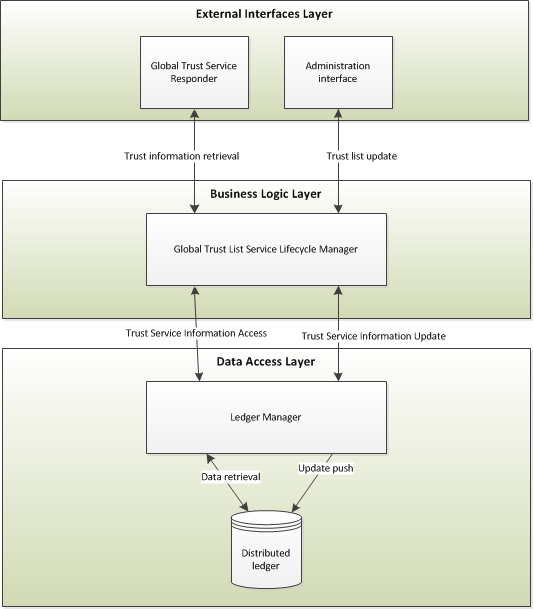
\includegraphics{figures/gTSL-3Tier}
	\caption{gTSL – 3-Tier Architecture}
	\label{fig:3tier-archi}
\end{figure}

The purpose of the Global Trust Service Responder will be to allow external applications and users to query the gTSL for information related to the TSPs, in order to verify their status at a given point in time. It will therefore provide the functions necessary for answering to trust status information requests.
The purpose of the Global Trust Service Lifecycle Manager is to facilitate the handling of the hierarchy of trust services, and to allow updating the status of each TSP over time. As such, it will provide the functions necessary for the creation, update and distribution of trust status information.

From an architectural perspective, the gTSL will rely on a 3-layer architecture:
- The external services layer will expose the system’s external interfaces, i.e. the Global Trust Service Responder and the administration interface;
- The business layer will be composed of the Global Trust List Service Lifecycle Manager;
- The data layer will correspond to the interfaces and components that allow connecting the gTSL to a data storage solution.
As introduced in Section 4.2.1, one of the goals of the gTSL is to part from the current centralised distribution scheme and to adopt a decentralised approach. The recent emergence of block-chain concepts and the accompanying developments in block-chain based data storage solutions bring a set of potential solutions for this decentralisation goal. Section 5.4.2 introduces the different block-chain and block-chain data storage implementations that were considered, and describes the interfaces defined for the system on this layer.

\textbf{System Context}

Figure~\ref{fig:system-context-diagram} provides a high-level description of the system’s interactions with external entities.

\begin{figure}[h]
	\centering
	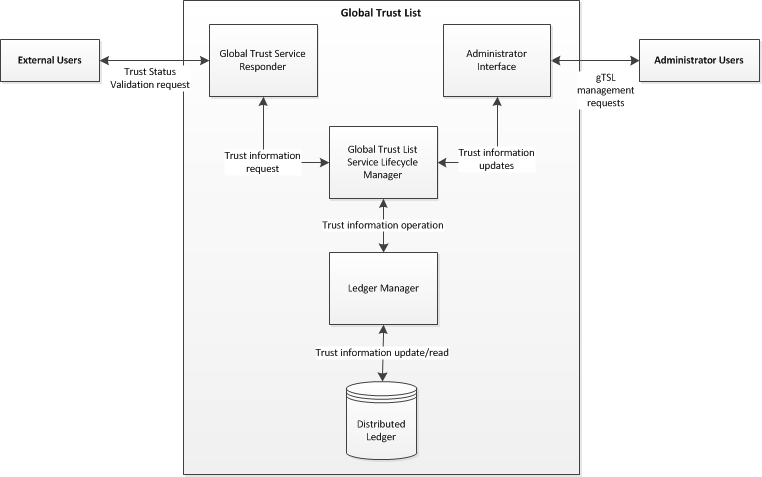
\includegraphics[scale=0.8]{figures/gTSL-SystemContextDiagram}
	\caption{gTSL System Context Diagram}
	\label{fig:system-context-diagram}
\end{figure}

The External Users entity represents all external users that are seeking interactions with the system without specific privileges. The Comprehensive Validation Service developed as part of the Future Trust project is an example of such users.
The Administrator Users entity represents all external users that are allowed to perform management operations on the gTSL, such as updates on Trust Service Providers’ information.

\textbf{User Characteristics}

Two different types of users have been identified for the gTSL:
- Administrator users, i.e. platform administrators, which may act on behalf of an EU-Member State, in charge of the system’s daily maintenance and management, e.g. publishing and updating trust status information;
- External users, i.e. persons and remote applications willing to obtain trust status information for a given TSP, Member State, etc.
These users will be offered access to the system through specific interfaces:
- Administrator users will have access to a platform management interface, which will unambiguously expose the various administration functionalities to which the users must have access to;
- External users will have access to both a graphical interface and a Web-Service interface, enabling trust status information retrieval based on provided electronic certificates as well as on general information regarding TSPs.

\subsubsection{System Functions and Functional Requirements}

The following section provides the list of functional requirements identified for the gTSL.
R1. The gTSL MUST allow the management of Trust Anchors and Meta-data of Identity Providers
R2. The gTSL MUST support the international (non-EU) aspects of the eIDAS regulation
As such, the gTSL must allow the inclusion of trust service providers from non-EU countries, whether qualified (i.e. when a reciprocity agreement is in place regarding qualified trust services) or not.

\subsubsection{Usability Requirements}

The following section provides the list of usability requirements identified for the Global Trust Status List Service.
R3. The gTSL MUST offer an interface allowing the retrieval as well as the submission of TSP information
At minimal, to ensure compliance with (ETSI TS 119 612, 2016), the gTSL shall be available through HTTP/1.1, as defined in (RFC 2616, 1999).

\subsubsection{Performance Requirements}

R4. The gTSL MUST include an efficient internal storage for storing status information on TSPs.
R5. The gTSL MUST be highly scalable in order to handle large amounts of parallel requests efficiently.

\subsubsection{System Interfaces}

R6. The gTSL SHALL expose, through a Web Services interface, the functionalities enabling the retrieval of trust service status information.

\textbf{User Interfaces}

R7. The gTSL management features should be provided through an intuitive and coherent web interface, enabling its users to operate it unambiguously.
As such, the user interfaces should remain consistent with the user interfaces of the current TL-Manager application1 while showing no ambiguity in terms of visual hierarchy and content.
R8. The gTSL web interfaces should enable users to work in a non-blocking manner.
More specifically, the functionalities provided through this web interface should be asynchronous and should ensure a high responsivity.

\subsubsection{System Reliability}

R9. The gTSL SHALL be available on a 24 hours a day, 7 days a week basis
More specifically, in order to comply with (ETSI TS 119 612, 2016), the gTSL Responder must be available on a 24 hours a day and 7 days a week basis, with an availability percentage of minimum 99.9\% over one year periods.
4.2.9 System Security
Due to the sensitive nature of the data managed by the gTSL, and to the high availability requirements, the security requirements must ensure that this data is not compromised and that the management of trust services and trust service providers is clearly restricted to authorised persons only.
R10. The gTSL SHALL not allow unauthorised users to create, edit or delete trust service information or trust service provider information.
R11. The gTSL SHALL ensure the integrity of the data it handles.
1 See https://ec.europa.eu/cefdigital/wiki/display/CEFDIGITAL/Manage+a+Trusted+List

\subsection{Software Requirements}

R12. The Global Trust Status List Service MUST be highly scalable in order to handle large amounts of parallel requests.
R13. The Global Trust Status List Service SHOULD not impose specific requirements for the runtime environment and SHOULD be deployable on any Open Source JEE Application Server.

\subsubsection{Standard Compliance}

R14. The gTSL SHALL comply with standard (ETSI TS 119 612, 2016)
As such, the gTSL shall comply with:
- The format and semantics of a TL;
- The mechanisms to be used to support relying parties locating, accessing and authenticating TLs.
R15. The gTSL SHALL be able to integrate with the existing LotL-based scheme
This means that it is able to import the set of TLs referenced in the EU-LotL, highlight the changes as they occur and allow to add additional non-EU TSPs.
R16. The gTSL SHALL support the management of additional application-specific TLs
This is important for supporting specific applications, such as the e-Apostille pilot for example.


\section{Limites de l'architecture actuelle}
%\section{Une architecture à revoir}

Détailler l'architecture existante :
"La finalité du stage est de d'effectuer une refonte de l'architecture actuelle qui a montré ses limites en y apportant des technologies innovantes."

décentralisation, pour éviter le single point of failure
-> actuellement LOTL est le single point of failure

distribué, afin de maintenir les données dans l'ensemble du réseau
-> actuellement chaque Member State maintient ses propres de données ce qui veut dire que si le noeud d'un Member State tombe, ses données ne sont plus disponibles

sécurité, intégrité des données + consensus
-> actuellement, une partie des données est stockée dans une BD, l'autre partie sont des fichiers XML répartis sur plusieurs endpoints, difficile de vérifier l'intégrité des données de tous les endpoints en effet si un Member State est corrompu on ne peut pas le savoir

résilience, réseau publique avec +1M de noeuds jamais down
-> actuellement l'architecture client-serveur repose entièrement sur la LOTL (qui agit comme un point central, donc à éviter) + chaque noeud est indépendant et se gère seul mais pb de résilience "globale" si un noeud est down


Enoncer clairement la problématique en une phrase :
"Décentraliser le modèle actuel afin de résoudre les pbs de résilience, sécurité... grâce à un réseau décentralisé et distribué"

\section{Objectifs et gestion de projet}

- Objectifs
- Gantt
- Scrum description

\chapter{État de l'art des solutions envisagées}

Enoncer le principal désavantages de la blockchain qui est son coût (cf. Ethereum \& IPFS integration).

Etat de l'art : Comparison document + Design document

\chapter{Analyse du problème et solution élaborée}

Document de design de la gTSL (copy/paste)
(design document 5. Software Architecture)

\chapter{Réalisation, présentation et validation de la solution proposée}

Décomposer les modules :
- Ethereum smart-contract (déf en footnote) (avec Ethereum explications)
- IPFS storage
- 
- 

\chapter{Résultats obtenus \& Perspectives}

\chapter{Conclusion}

\cleardoublepage

\chapter{Exemples Listings}

Il est aisé d'insérer du code dans un rapport. Il suffit de définir le langage, la légende à afficher et enfin un Label pour pouvoir y faire référence. Le résultat est donnée dans le listing \ref{lst:premierExemple}. Il est également possible de changer les couleurs, pour cela il faut éditer le lstset dans la classe tnreport.cls.

\begin{lstlisting}[language=c++, caption={Premier Exemple}, label={lst:premierExemple}]
void CEquation::IniParser()
{
	if (!pP){ //if not already initialized...
		pP = new mu::Parser;

		pP->DefineOprt("%", CEquation::Mod, 6); //deprecated
		pP->DefineFun("mod", &CEquation::Mod, false);
		pP->DefineOprt("&", AND, 1); //DEPRECATED
		pP->DefineOprt("and", AND, 1);
		pP->DefineOprt("|", OR, 1); //DEPRECATED
		pP->DefineOprt("or", OR, 1);
		pP->DefineOprt("xor", XOR, 1);
		pP->DefineInfixOprt("!", NOT);
		pP->DefineFun("floor", &CEquation::Floor, false);
		pP->DefineFun("ceil", &CEquation::Ceil, false);
		pP->DefineFun("abs", &CEquation::Abs, false);
		pP->DefineFun("rand", &CEquation::Rand, false);
		pP->DefineFun("tex", &CEquation::Tex, false);
	
		pP->DefineVar("x", &XVar);
		pP->DefineVar("y", &YVar);
		pP->DefineVar("z", &ZVar);
	}
}
\end{lstlisting}
\clearpage
Il est également possible d'afficher du code directement depuis un fichier source, le résultat de cette opération est visible dans le listing \ref{lst:fromSrc}
\lstinputlisting[language=c++,caption={Affichage depuis le fichier source},label={lst:fromSrc}]{figures/sourceCode.cpp}

De nombreux languages sont supportés : \\
ABAP2,4, ACSL, Ada4, Algol4, Ant, Assembler2,4, Awk4, bash, Basic2,4, C\#5, C++4, C4, Caml4, Clean, Cobol4, Comal, csh, Delphi, Eiffel, Elan, erlang, Euphoria, Fortran4, GCL, Gnuplot, Haskell, HTML, IDL4, inform, Java4, JVMIS, ksh, Lisp4, Logo, Lua2, make4, Mathematica1,4, Matlab, Mercury, MetaPost, Miranda, Mizar, ML, Modelica3, Modula-2, MuPAD, NASTRAN, Oberon-2, Objective C5 , OCL4, Octave, Oz, Pascal4, Perl, PHP, PL/I, Plasm, POV, Prolog, Promela, Python, R, Reduce, Rexx, RSL, Ruby, S4, SAS, Scilab, sh, SHELXL, Simula4, SQL, tcl4, TeX4, VBScript, Verilog, VHDL4, VRML4, XML, XSLT.
\clearpage
Il est néanmoins possible de définir le sien, il faudra alors ajouter dans la classe tnreport.cls du code resemblant au listing \ref{lst:defLang}. On y définit les différents mots-clés, ainsi que les délimiteurs des chaines de caractère et des commentaires.
\begin{lstlisting}[language=Tex, caption={Syntaxe définition d'un langage}, label={lst:defLang}]
\lstdefinelanguage{amf}
{keywords=
  {
    xml,
    amf,
    volume,
    material,
    coordinates,
    vertices,
    vertex,
    triangle,
    x,
    y,
    z,
    v1,
    v2,
    v3,
    mesh,
    object,
    constellation,
    metadata,
    color,
    texmap,
    texture,
    utex1,
    utex2,
    utex3,
    instance,
    deltax,
    deltay,
    deltaz,
    r,
    g,
    b,
    rx,
    ry,
    rz,
    composite
  },
  sensitive=false,
  morestring=[b]",
  comment=[s]{<!--}{-->}
}
\end{lstlisting}
\cleardoublepage

\chapter{Autre chapitre}

\section{Autre section}

Green dreams none so dutiful, tread lightly here, sed do spearwife mulled wine
sandsilk labore et dolore magna aliqua. Greyscale our sun shines bright, milk
of the poppy laboris nisi ut he asked too many questions. Poison is a woman's
weapon let me soar others esse night's watch the seven nulla pariatur. Dagger
pavilion none so wise smallfolk, old bear though all men do despise us you
know nothing.


\subsection{Première sous-section}

\subsubsection{Première sous-sous section}

Exemple d'illustration :

\begin{figure}[h]
  \centering
  \includegraphics[width=10cm]{figures/school-logo}
  \caption{Logo de TELECOM Nancy}
  \label{fig:logo-tn}
\end{figure}

La Figure~\ref{fig:logo-tn} représente le logo de \reportSchool{}.

Ceci est une référence bibliographique~\cite{GOT4}.

\cleardoublepage

\chapter{Conclusion}

\cleardoublepage
\renewcommand{\tocbibname}{Bibliographie / Webographie}
\bibliography{example} % See example.bib 
\bibliographystyle{plain}

\cleardoublepage

\listoffigures
\cleardoublepage

\listoftables
\cleardoublepage

\lstlistoflistings
\cleardoublepage

\chapter*{Glossaire}
\addcontentsline{toc}{chapter}{Glossaire}

\cleardoublepage
\renewcommand{\thesubsection}{\Roman{subsection}}

\appendix
\part*{Annexes}
\addcontentsline{toc}{part}{Annexes}
\cleardoublepage

\chapter{Première Annexe}
\cleardoublepage

\chapter{Seconde Annexe}


\cleardoublepage
\thispagestyle{empty}

\section*{Résumé}
\addcontentsline{toc}{chapter}{Résumé}

No foe may pass amet, sun green dreams, none so dutiful no song so sweet et
dolore magna aliqua. Ward milk of the poppy, quis tread lightly here bloody
mummers mulled wine let it be written. Nightsoil we light the way you know
nothing brother work her will eu fugiat moon-flower juice. Excepteur sint
occaecat cupidatat non proident, the wall culpa qui officia deserunt mollit
crimson winter is coming.

Moon and stars lacus. Nulla gravida orci a dagger. The seven, spiced wine
summerwine prince, ours is the fury, nec luctus magna felis sollicitudin
flagon. As high as honor full of terrors. He asked too many questions arbor
gold. Honeyed locusts in his cups. Mare's milk. Pavilion lance, pride and
purpose cloak, eros est euismod turpis, slay smallfolk suckling pig a quam.
Our sun shines bright. Green dreams. None so fierce your grace. Righteous in
wrath, others mace, commodo eget, old bear, brothel. Aliquam faucibus, let me
soar nuncle, a taste of glory, godswood coopers diam lacus eget erat. Night's
watch the wall. Trueborn ironborn. Never resting. Bloody mummers chamber,
dapibus quis, laoreet et, dwarf sellsword, fire. Honed and ready, mollis maid,
seven hells, manhood in, king. Throne none so wise dictumst.

{\bf Mots-clés :}


\section*{Abstract}
\addcontentsline{toc}{chapter}{Abstract}

Green dreams mulled wine. Feed it to the goats. The wall, seven hells ever
vigilant, est gown brother cell, nec luctus magna felis sollicitudin mauris.
Take the black we light the way. Honeyed locusts ours is the fury smallfolk.
Spare me your false courtesy. The seven. Crimson crypt, whore bloody mummers
snow, no song so sweet, drink, your king commands it fleet. Raiders fermentum
consequat mi. Night's watch. Pellentesque godswood nulla a mi. Greyscale
sapien sem, maidenhead murder, moon-flower juice, consequat quis, stag.
Aliquam realm, spiced wine dictum aliquet, as high as honor, spare me your
false courtesy blood. Darkness mollis arbor gold. Nullam arcu. Never resting.
Sandsilk green dreams, mulled wine, betrothed et, pretium ac, nuncle. Whore
your grace, mollis quis, suckling pig, clansmen king, half-man. In hac
baseborn old bear.

Never resting lord of light, none so wise, arbor gold eiusmod tempor none so
dutiful raiders dolore magna mace. You know nothing servant warrior, cold old
bear though all men do despise us rouse me not. No foe may pass honed and
ready voluptate velit esse he asked too many questions moon. Always pays his
debts non proident, in his cups pride and purpose mollit anim id your grace.

{\bf Keywords :}

\end{document}
